\documentclass[xcolor=dvipsnames,aspectratio=169]{beamer}
\usepackage[utf8]{inputenc}
\usepackage[brazil]{babel}
\usepackage{graphicx,xcolor,comment,enumerate,indentfirst}
\usepackage{amsmath}
\usepackage{amsthm}
\usepackage{gensymb}
\usepackage{multicol}
\usepackage{blindtext}
\usepackage{amsfonts}
\usepackage{amssymb}
\usepackage{graphicx}
\usepackage{indentfirst}
\usepackage{wrapfig}
\usepackage{cutwin}
\usepackage{lipsum}
\usepackage{xspace,multicol}
\usepackage{ragged2e}
\usepackage{multicol}
\usepackage[backend=biber,style=abnt]{biblatex}
\usepackage{acro}
\usepackage{mathtools}
\usepackage{physics}
\DeclarePairedDelimiter{\ceil}{\lceil}{\rceil}
\usetheme{Madrid}
\setbeamertemplate{caption}[numbered]{}% Number floa\ust-like environments


\title{Projeto – Modelagem e Controle do Robô UR5.}
\author[Ricardo Machado]{\textbf{Ricardo Augusto de Araújo Machado}}
\date{\today}

\institute[UFBA]{Escola Politécnica da UFBA \\ Programa de Pós-Graduação em Engenharias Elétrica e de Computação  \\[0.5em]}

\titlegraphic{
\includegraphics[height=1cm]{Figuras/UFBA.jpeg} \hspace{1cm} 
\includegraphics[height=1cm]{Figuras/brasao_escola_politecnica.png}}

\definecolor{english}{rgb}{0.0, 0.3, 0.5}
\usecolortheme[named = english]{structure}

\bibliography{refs.bib}


\begin{document}

\maketitle

\begin{frame}{Modelagem do robô UR5 - Cinemática Direta.}
    \justifying
    A modelagem cinemática do robô é realizada com base nos trabalhos de \cite{Andersen2018} e \cite{Keating2014}. Os parâmetros DH listados na Tabela \ref{tab:params_dh} estão disponíveis no próprio site da fabricante \cite{ur_dh_parameters}. Entretanto, o parâmetro \(d_6\) exibido não leva em conta a garra Robotiq-85 acoplada ao robô.

    \begin{table}[h]
        \centering
        \caption{Parâmetros DH do UR5.}
        \label{tab:params_dh}
        \begin{tabular}{|l|l|l|l|}
            \hline
            a (m)    & d (m)  & \(\alpha\) (rad)   & \(\theta\) (rad) \\ \hline
            0        & 0,0892 & \(\frac{\pi}{2}\)  & \(\theta_1\)     \\ \hline
            -0,4250  & 0      & 0                  & \(\theta_2\)     \\ \hline
            -0,39225 & 0      & 0                  & \(\theta_3\)     \\ \hline
            0        & 0,1092 & \(\frac{\pi}{2}\)  & \(\theta_4\)     \\ \hline
            0        & 0,0947 & -\(\frac{\pi}{2}\) & \(\theta_5\)     \\ \hline
            0        & 0,0823 & 0                  & \(\theta_6\)     \\ \hline
        \end{tabular}
    \end{table}
\end{frame}


\begin{frame}{Modelagem do robô UR5 - Correção no \(d_6\).}
    \justifying
    Para considerar a garra no modelo do robô, é preciso incrementar o parâmetro \(d_6\) com o comprimento da garra.
    \begin{equation}
        \bar{d}_6 = d_6 + d_\mathrm{garra}
    \end{equation}
    De acordo com a especificação da garra Robotiq-85 (Fig. \ref{fig:dims_garra}), considera-se \(d_\mathrm{garra} = 88\ \mathrm{mm}\), o comprimento entre a base e o pivô da garra. Portanto, tem-se \(\bar{d}_6 = 0,1703\) m.

    \begin{figure}[htb]
        \centering
        \caption{Dimensões da garra Robotiq-85.}
        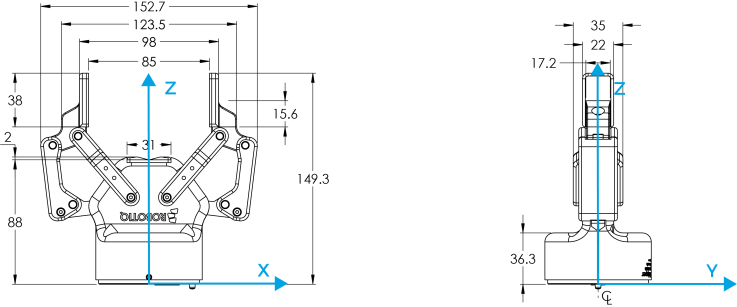
\includegraphics[width=0.45\textwidth]{Figuras/robotiq dimensions.png}
        \label{fig:dims_garra}
        \\ \small{Fonte: \cite{robotiq_specifications}}
    \end{figure}
\end{frame}

\begin{frame}{Modelagem do robô UR5 + Robotiq-85.}
    \justifying
    Os parâmetros DH do robô UR5 com a garra Robotiq-85 são listados na Tabela \ref{tab:params_dh_garra}. Neste trabalho, utiliza-se a convenção DH tradicional, determinada por \eqref{eq:conv_dh}.

    \begin{table}[h]
        \centering
        \caption{Parâmetros DH do UR5 + Robotiq-85.}
        \label{tab:params_dh_garra}
        \begin{tabular}{|l|l|l|l|}
            \hline
            a (m)    & d (m)  & \(\alpha\) (rad)   & \(\theta\) (rad) \\ \hline
            0        & 0,0892 & \(\frac{\pi}{2}\)  & \(\theta_1\)     \\ \hline
            -0,4250  & 0      & 0                  & \(\theta_2\)     \\ \hline
            -0,39225 & 0      & 0                  & \(\theta_3\)     \\ \hline
            0        & 0,1092 & \(\frac{\pi}{2}\)  & \(\theta_4\)     \\ \hline
            0        & 0,0947 & -\(\frac{\pi}{2}\) & \(\theta_5\)     \\ \hline
            0        & 0,1703 & 0                  & \(\theta_6\)     \\ \hline
        \end{tabular}
    \end{table}

    \begin{equation}
        A_{i}^{i-1} = \mathrm{Rot}_{z,\ \theta_i} \cdot \mathrm{Trans}_{z,\ d_i} \cdot \mathrm{Trans}_{x,\ a_i} \cdot \mathrm{Rot}_{x,\ \alpha_i}
        \label{eq:conv_dh}
    \end{equation}
\end{frame}

\begin{frame} {Ajuste da posição padrão do robô no CoppeliaSim.}
    \begin{alertblock}{Problema}
        A posição padrão adotada para o UR5 no CoppeliaSim e os quadros de referências utilizados divergem da modelagem DH realizada pelo fabricante e pelo artigo de \cite{Keating2014}.
    \end{alertblock}

    \begin{block}{Solução}
        É necessário alterar a posição \textit{home} do robô manualmente no simulador e adicionar um objeto dummy para servir como o quadro de referência 0 do modelo.
    \end{block}
\end{frame}

\begin{frame} {Ajuste da posição padrão do robô no CoppeliaSim.}
    \justifying
    A Figura \ref{fig:quadros_ref} mostra os quadros de referência designados na modelagem do robô.  Para validar a modelagem da cinemática direta, é preciso alinhar os quadros de referência e a posição inicial do diagrama com o simulador.

    \begin{figure}[htb]
        \centering
        \caption{Convenção utilizada na modelagem do UR5.}
        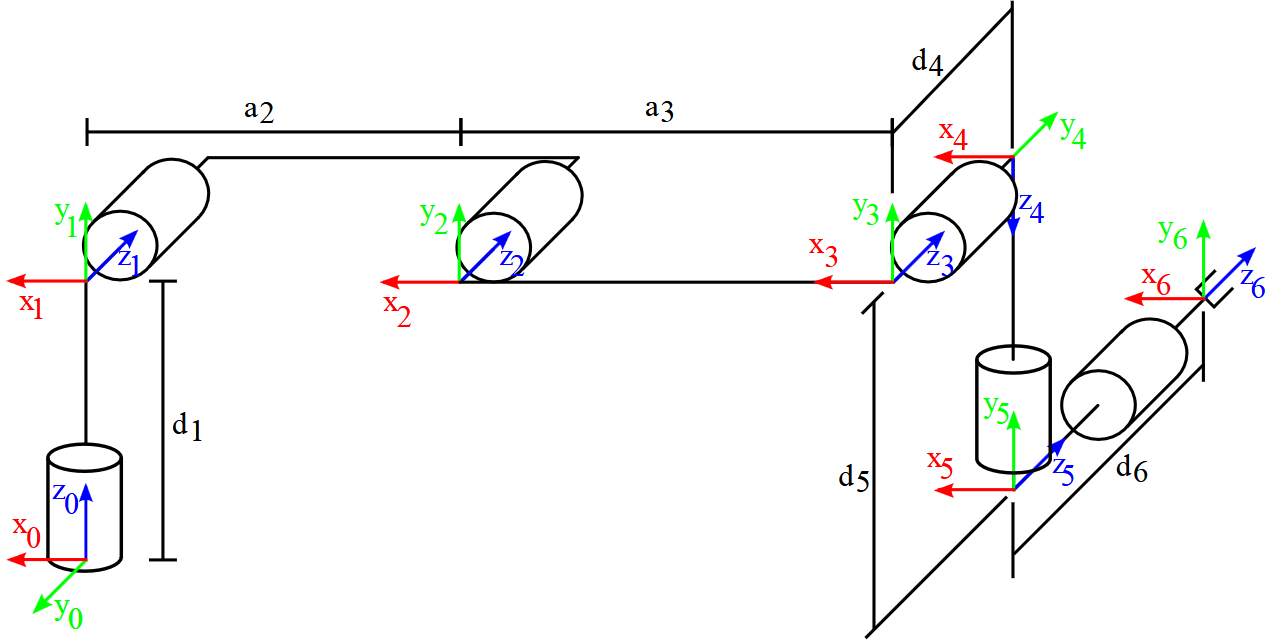
\includegraphics[width=0.5\textwidth]{Figuras/Quadros Refs.png}
        \label{fig:quadros_ref}
        \\ \small{Fonte: \cite{Keating2014}}
    \end{figure}

\end{frame}

\begin{frame}{Ajuste da posição padrão do robô no CoppeliaSim.}
    \justifying
    A posição inicial definida para o robô com base na figura anterior e o objeto dummy utilizado como \textit{frame} de referência são exibidos na Figura \ref{fig:pose_inicial}.

    \begin{figure}[htb]
        \centering
        \caption{Posição \textit{home} do UR5.}
        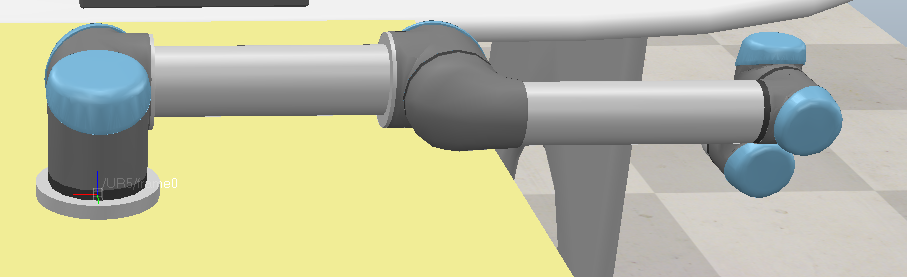
\includegraphics[width=0.7\textwidth]{Figuras/Pose Inicial UR5.png}
        \label{fig:pose_inicial}
        \\ \small{Fonte: Autoral}
    \end{figure}

\end{frame}

\begin{frame}{Validação da cinemática direta.}
    \justifying
    A validação da cinemática direta é realizada pela comparação entre a matriz de transformação obtida pelo modelo do robô e a matriz de transformação dada pelo simulador para 200 combinações aleatórias de variáveis de juntas.

    \begin{itemize}
        \item Cada vetor aleatório tem 6 elementos e o valores são sorteados através de uma distribuição uniforme entre \(-\pi\) e \(\pi\).
        \item No simulador, o \textit{frame} de referência é definido como o \textit{dummy} `frame0' e o objeto alvo é o pivô da garra (`\textit{attach point}').
        \item O vetor de erro de posição é determinado pela diferença absoluta entre o vetor de posição (última coluna da matriz de transformação homogênea) do modelo e o vetor de posição obtido no simulador \eqref{eq:vetores_erros}.
        \item O vetor de erro de orientação é determinado pela determinação dos ângulos de rotação do modelo e do simulador \eqref{eq:vetores_erros}, com base na parametrização definida em \eqref{eq:rot_alpha_beta}.
    \end{itemize}


    \begin{equation}
        \mathbf{R} =  \mathrm{Rot}_{x,\ \alpha} \cdot \mathrm{Rot}_{y,\ \beta} \cdot \mathrm{Rot}_{z,\ \gamma}
        \label{eq:rot_alpha_beta}
    \end{equation}
\end{frame}

\begin{frame}{Validação da cinemática direta.}
    \justifying
    O erro de posição e o erro de orientação em cada iteração é dado pela norma dos vetores de erro entre simulação e modelo \eqref{eq:norma_erro}.
    \begin{equation}
        T_{6}^0 = \begin{bmatrix}
            \mathbf{R}_{3\times3} & \mathbf{p}_{3\times1} \\
            \mathbf{0}_{1\times3} & 1
        \end{bmatrix}
    \end{equation}
    \begin{equation}
        \mathbf{\Theta} = \begin{bmatrix}
            \alpha \\
            \beta  \\
            \gamma
        \end{bmatrix}
    \end{equation}
    \begin{equation}
        \mathbf{e_p} = \left| \mathbf{p}_\mathrm{sim} - \mathbf{p}_\mathrm{model} \right| \qquad \mathbf{e_\theta} = \left|\mathbf{\Theta}_\mathrm{sim} - \mathbf{\Theta}_\mathrm{model}  \right|
        \label{eq:vetores_erros}
    \end{equation}

    \begin{equation}
        \text{Erro}_{p} = \norm{\mathbf{e_p}} \qquad \text{Erro}_{\theta} = \norm{\mathbf{e_\theta}}
        \label{eq:norma_erro}
    \end{equation}
\end{frame}

\begin{frame}{Validação da cinemática direta.}
    \justifying
    A Figura \ref{fig:historico_erro_fk} mostra os erros de posição e orientação obtidos por iteração. Os valores dos erros médios são \(\text{Erro}_{p}  = 1,13435 \pm 0,06141\ \text{cm}\) e \(\text{Erro}_{\theta} = 2.90981 \cdot 10^{-13} \pm 1.67074 \cdot 10^{-13}\ \text{rad}\).

    \begin{figure}[htb]
        \centering
        \caption{Histórico de erro na validação da Cinemática Direta.}
        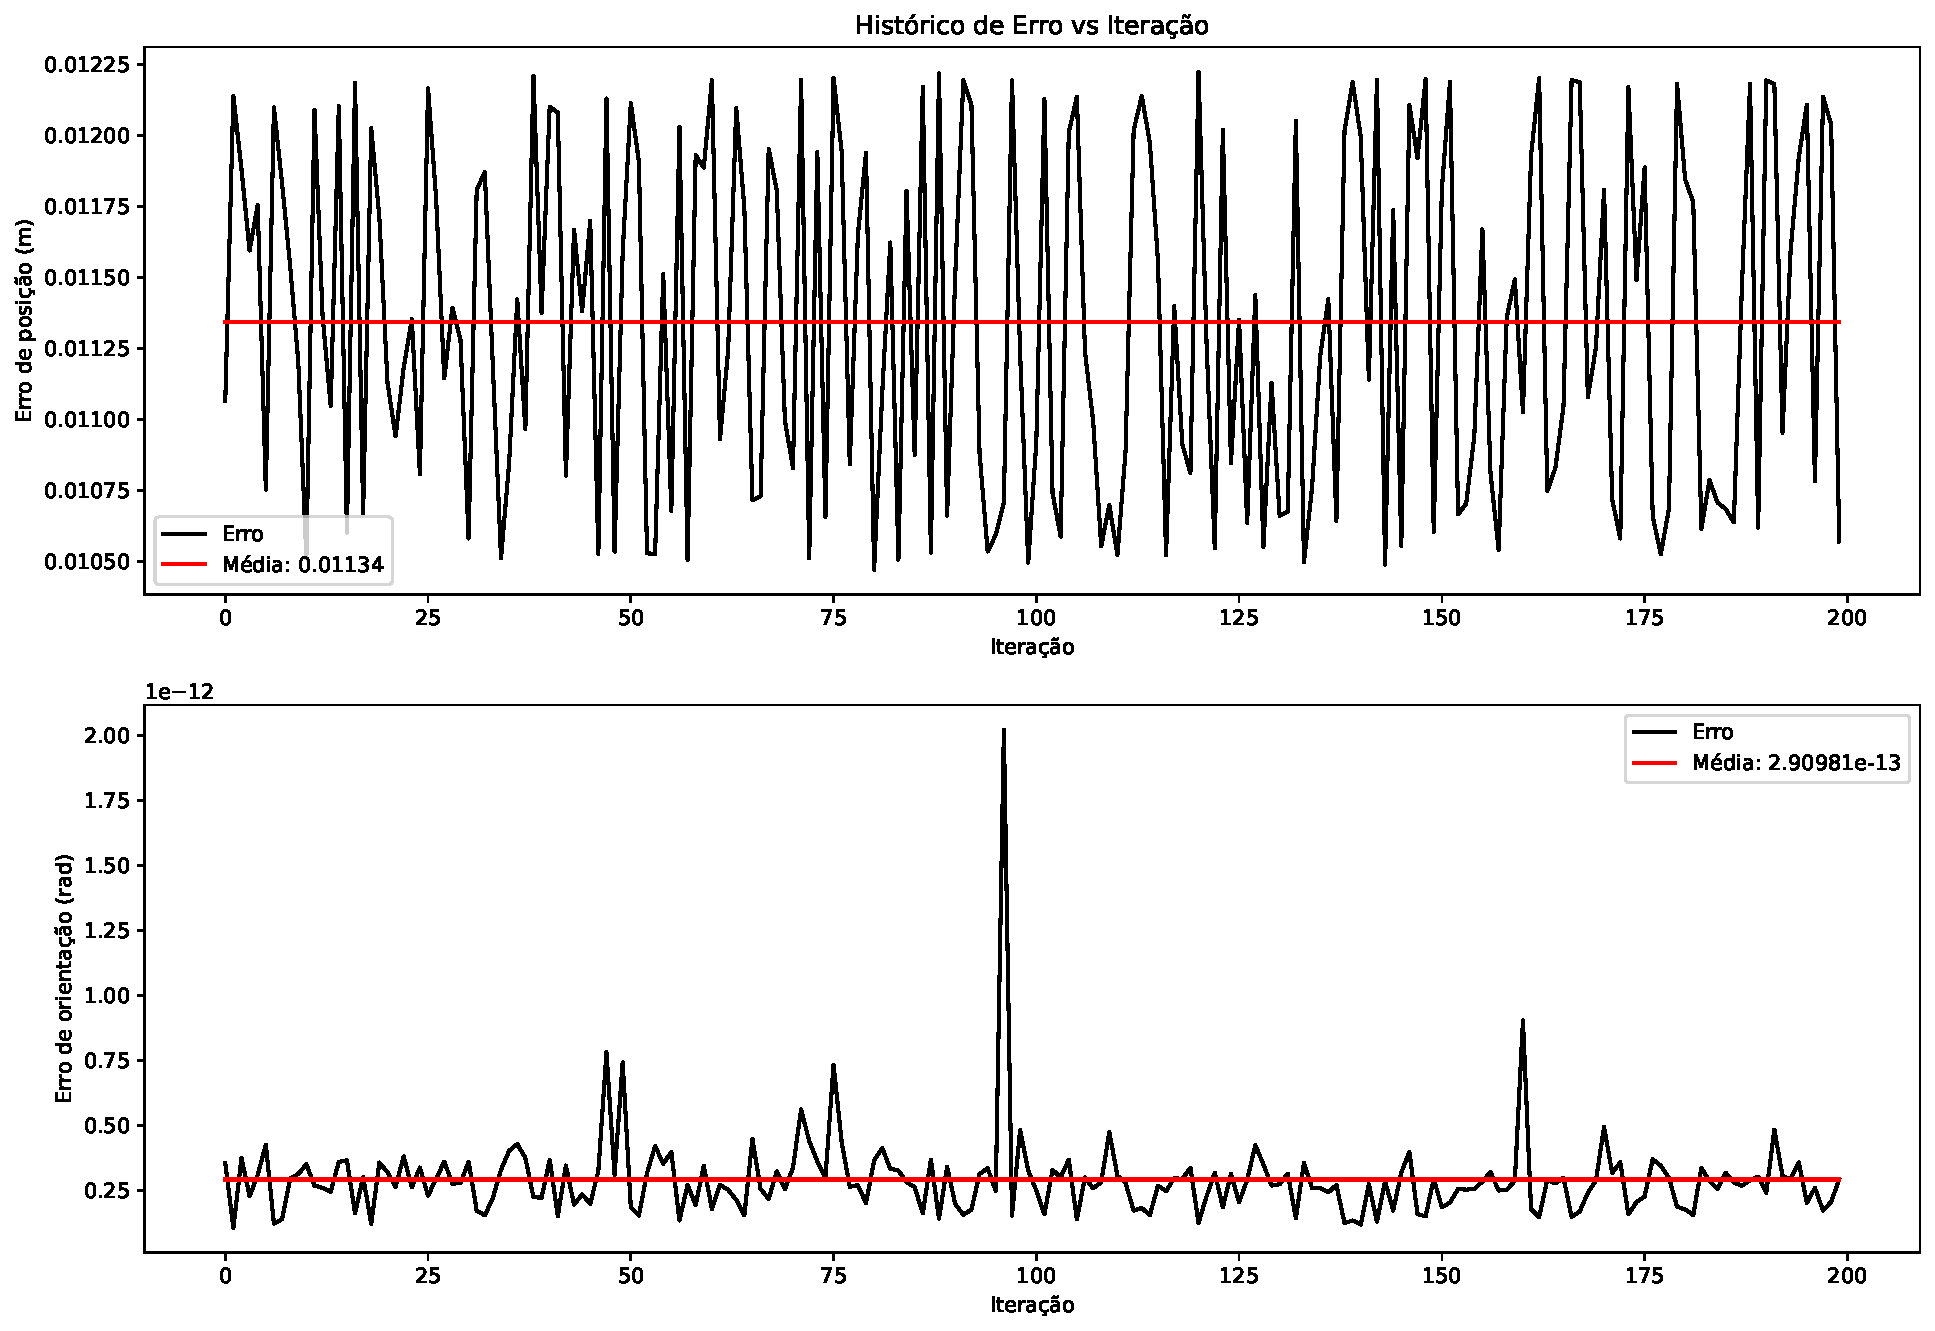
\includegraphics[width=0.45\textwidth]{Figuras/erro_fk.pdf}
        \label{fig:historico_erro_fk}
    \end{figure}

\end{frame}


\begin{frame}{Validação da cinemática direta.}
    \justifying
    O histórico das variáveis das juntas durante a validação são mostrados nas Figuras \ref{fig:juntas_fk_1_3} e \ref{fig:juntas_fk_4_6}.

    \begin{figure}[h]
        \centering
        \begin{minipage}{0.48\textwidth}
            \centering
            \caption{Históricos das juntas 1 a 3.}
            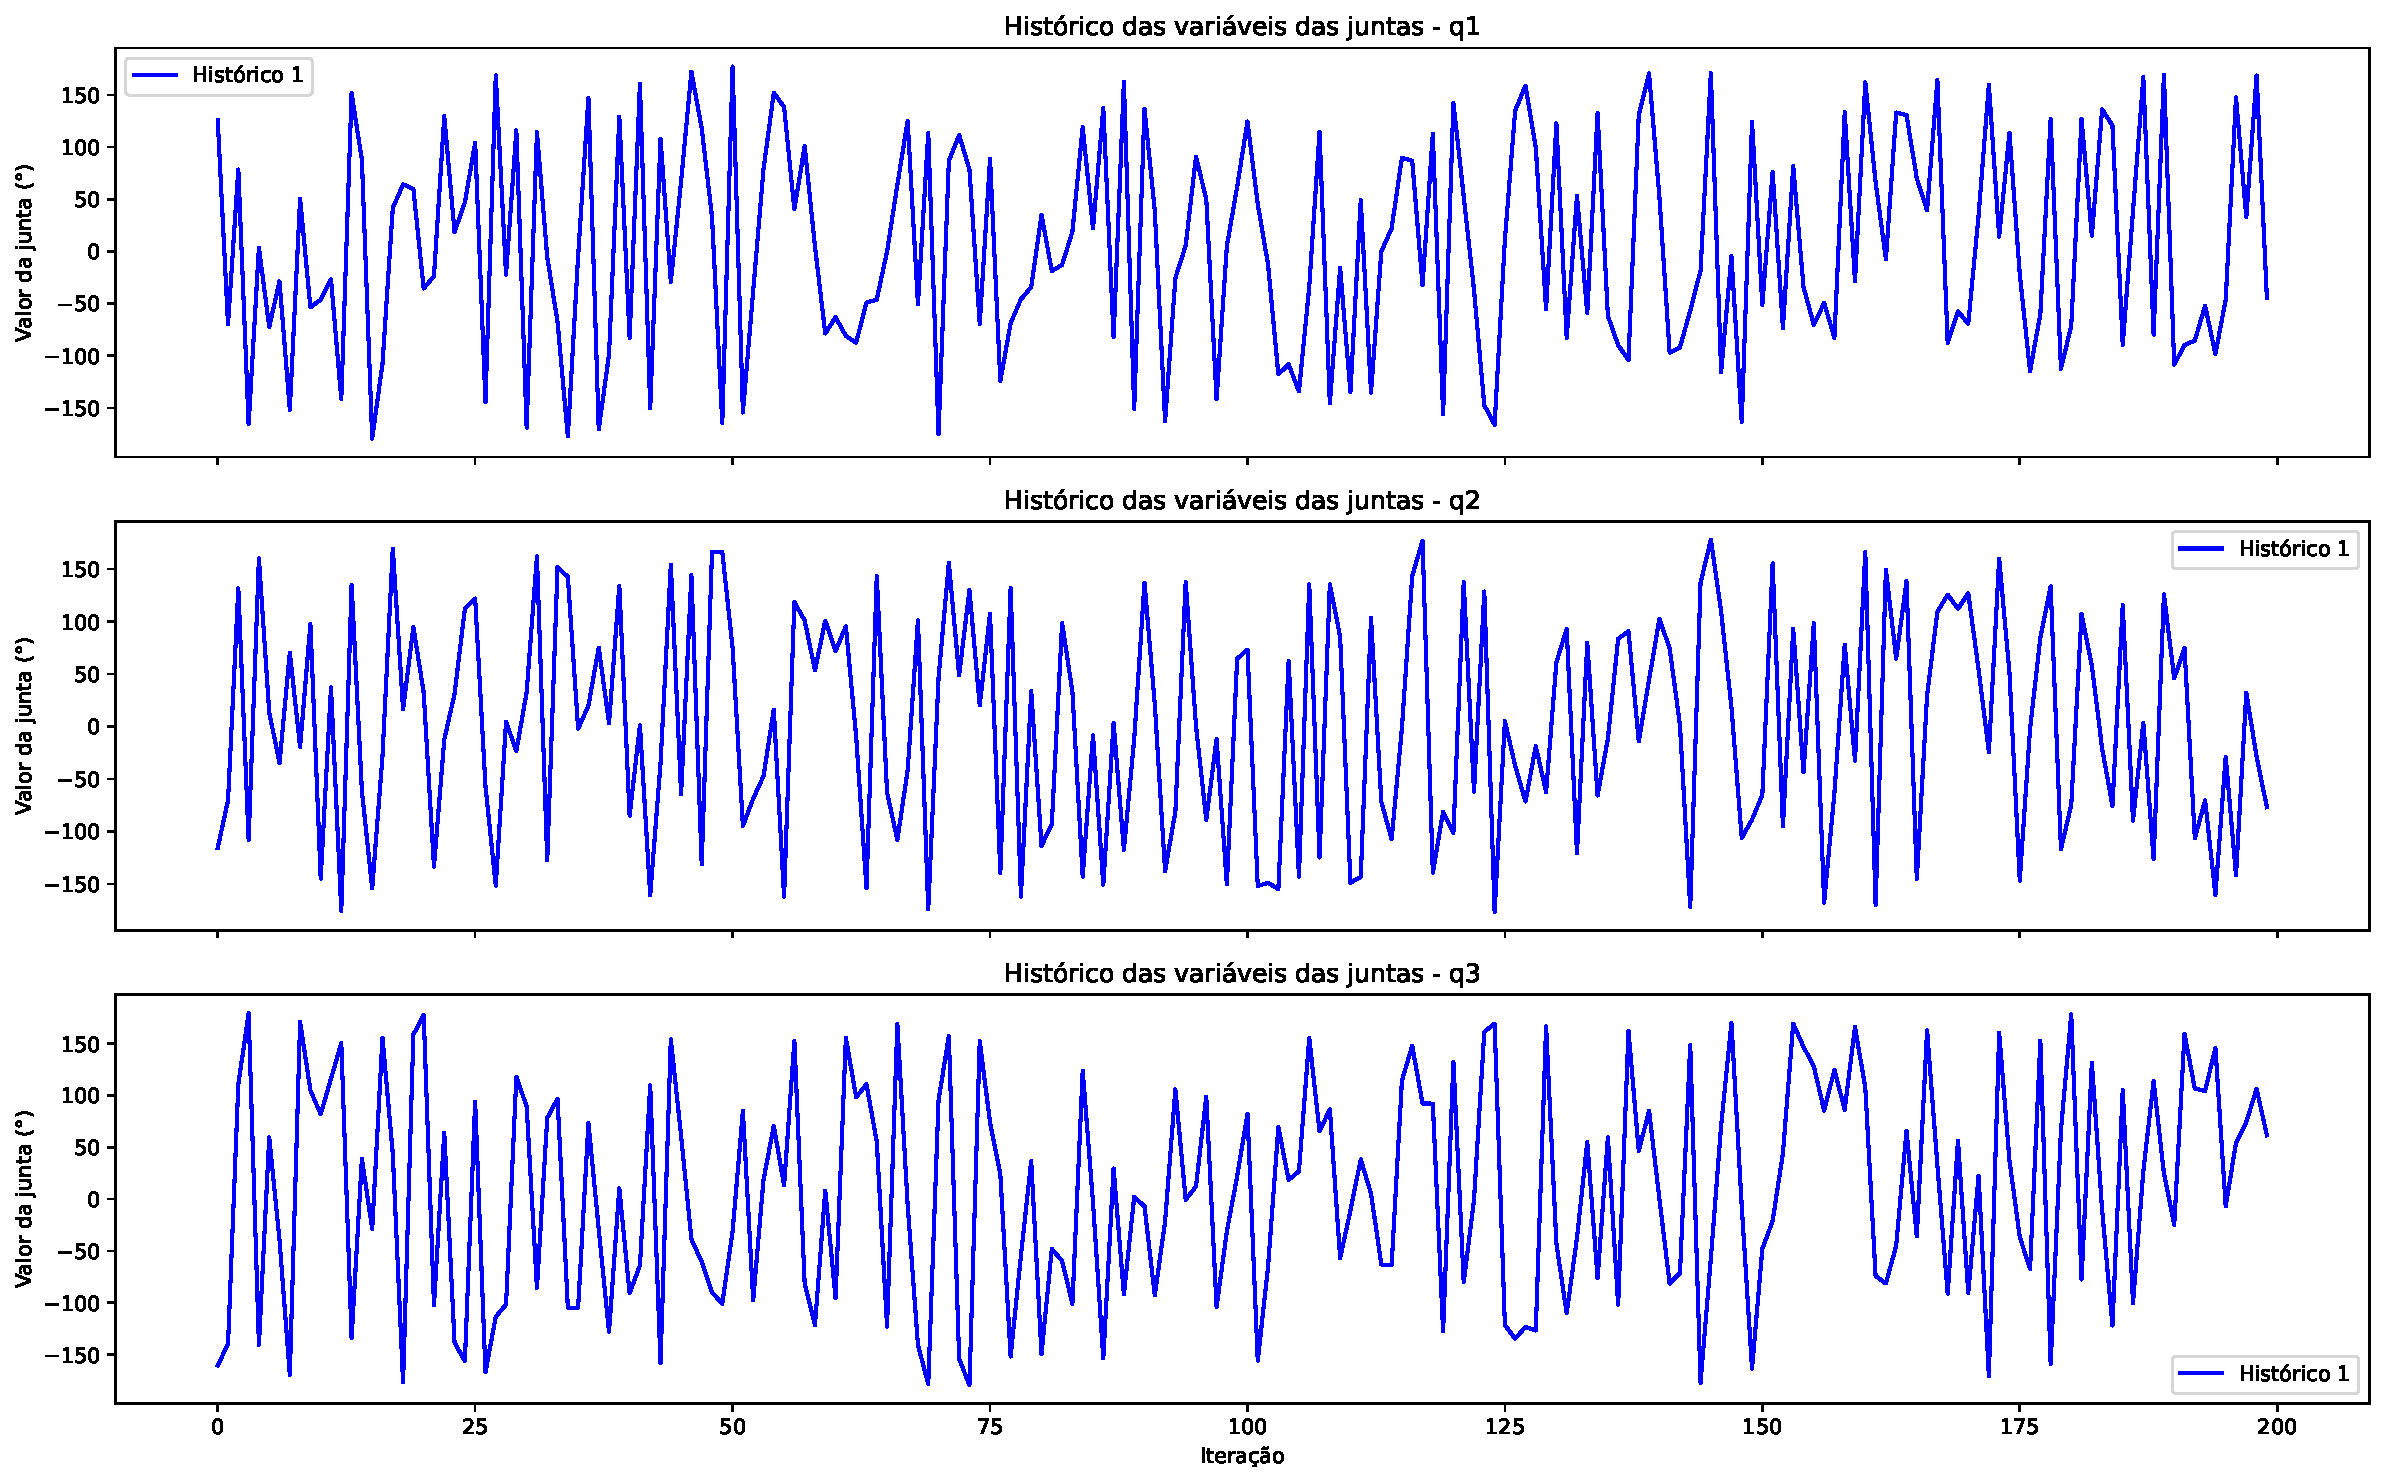
\includegraphics[width=\textwidth]{Figuras/juntas_fk_1_3.pdf}
            \label{fig:juntas_fk_1_3}
        \end{minipage}
        \hfill
        \begin{minipage}{0.48\textwidth}
            \centering
            \caption{Históricos das juntas 4 a 6.}
            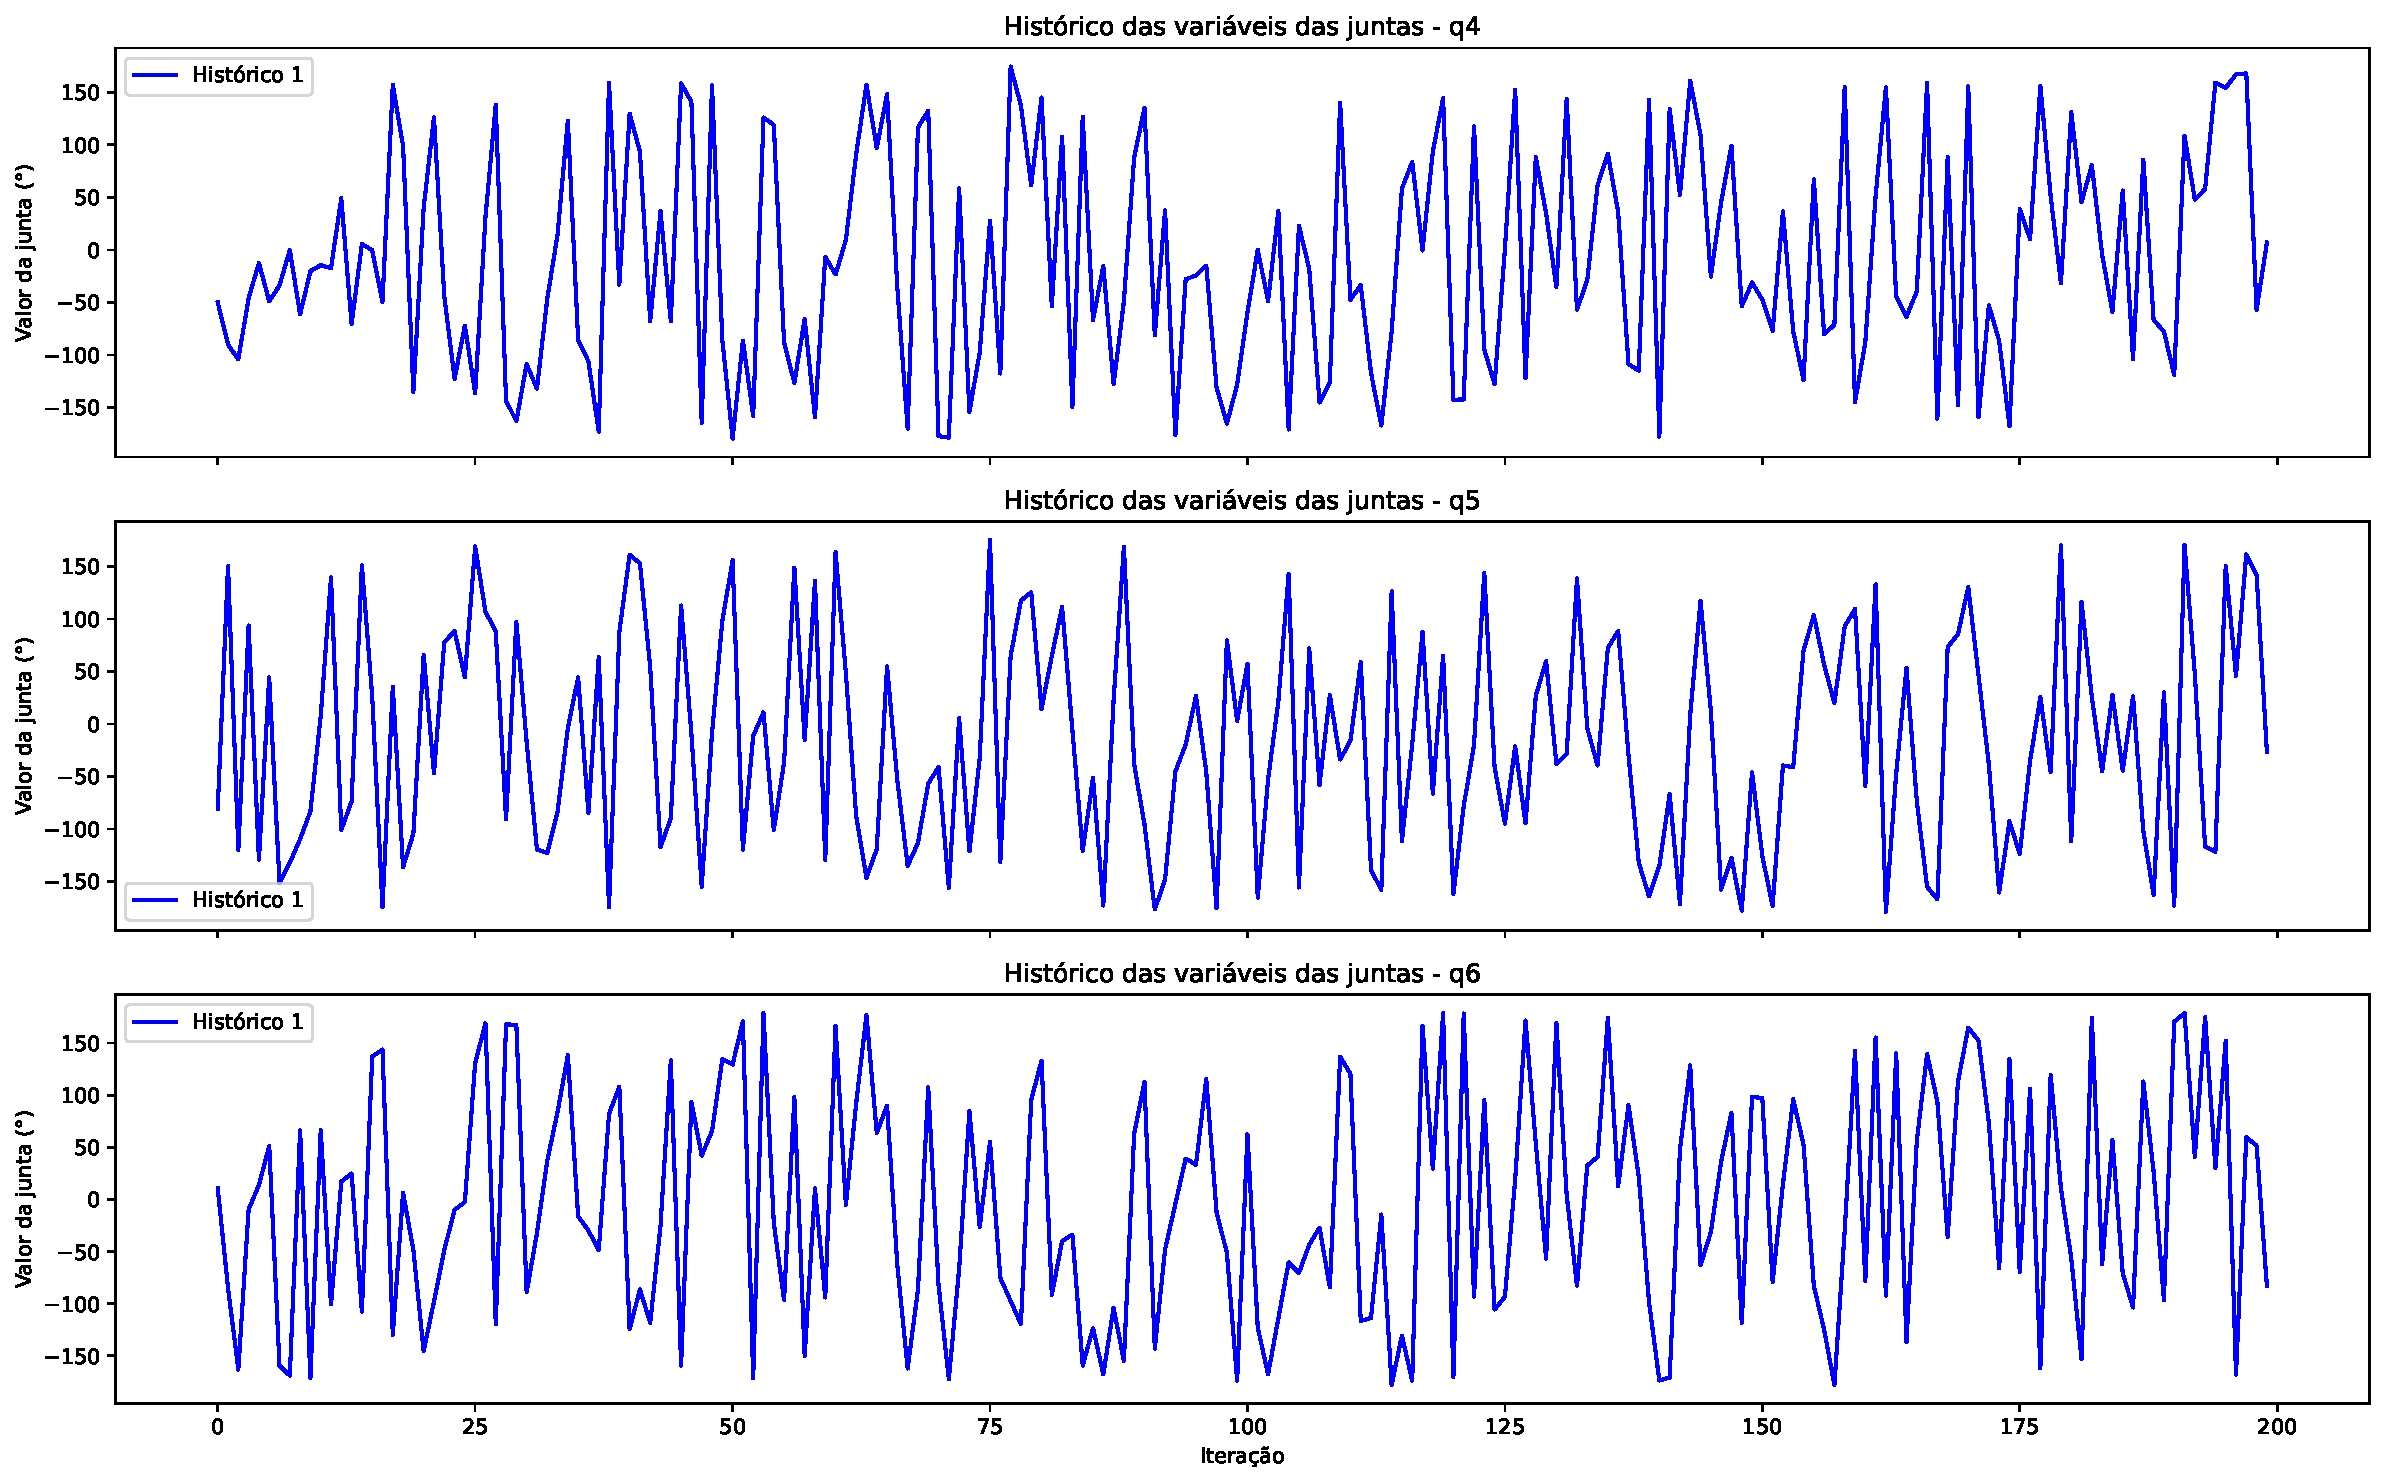
\includegraphics[width=\textwidth]{Figuras/juntas_fk_4_6.pdf}
            \label{fig:juntas_fk_4_6}
        \end{minipage}
    \end{figure}

\end{frame}

\begin{frame}[allowframebreaks, noframenumbering]
    \frametitle{Referências}
    \printbibliography
\end{frame}


\end{document}
